\documentclass[a4paper]{book}

% packages % 
\usepackage[utf8]{inputenc} 
\usepackage{fvextra}
\usepackage{csquotes}
\usepackage[french, italian, spanish, english]{babel}
\usepackage[T1]{fontenc}   
\usepackage{color}  
\usepackage{amsmath, dsfont, amssymb, amsthm, stmaryrd}
\usepackage[style=alphabetic]{biblatex}
\usepackage{enumitem}
\usepackage[hidelinks]{hyperref}

% graphics %
\usepackage{graphicx}
\graphicspath{ {./images/} }

% environments %
\newtheorem{theorem}{Theorem}[section]
\newtheorem{corollary}{Corollary}[theorem]
\newtheorem{lemma}[theorem]{Lemma}

\theoremstyle{definition}
\newtheorem{definition}{Definition}[section]

\theoremstyle{remark}
\newtheorem*{remark}{Remark}
\newtheorem*{example}{Example}



% bibliography %
\bibliography{bibliography} 

\begin{document}

% title %
\title{Statistical field theory and applications}
\author{Buisine Léo\\Ecole Normale Superieure of Paris}
\maketitle

\tableofcontents

\chapter{Introduction}
Email adress: adam.nahum@phys.ens.fr \newline 
TDman: xiangyu.cao@phys.ens.fr (he also has a website) \par  \bigskip 

Books 
\begin{enumerate}
    \item Cardy, but condensed
\end{enumerate} \bigskip

Statistical field theory: just applying statistical mechanics idea to systems 

\section{Renormalization group (preview)}

Very general tool from 20th century physics to understand complex systems (spatially extended and many degrees of freedom). Explains why QFT is so powerful in high energy physics and statistical physics 

\begin{example}
    Classical lattice models, modelizes magnetism for example
    \begin{equation}
        Z = \sum_{\{S\}e-\beta E(s)} \qquad \beta = \frac{1}{k_B T}
    \end{equation}
\end{example}
\begin{example}
    Statistical field theory
    \begin{equation}
        Z = \int \mathcal{D}\varphi(x) e^{-\mathcal{H}(\varphi)}
    \end{equation}
\end{example}
\begin{example}
    Qauntum lattice model, chain with spin up or down for example 
    \begin{equation}
        Z = \text{Tr}(e^{-\beta H})
    \end{equation}
\end{example}
\begin{example}
    Quantum field theories
    \begin{equation}
        Z = \int \mathcal{D}\varphi(x, t)e^{-\mathcal{S}(\varphi)}
    \end{equation}
    with 
    \begin{equation}
        \mathcal{S}(\varphi) = \int \text{d}^d x \int^\beta_0 \text{d}t [(\partial_t\varphi)^2 + (\triangledown  \varphi)^2\dots ]
    \end{equation}
\end{example}

\underline{Renormalization group}: \newline 
Key idea: The useful theoretical description is different at different scales. \newline 
Aim: understand how description changes as we "zoom out".\newline 
Objective of finding a universal description and forgetting useless information\par \medskip 

A simple SFT and complicated microscopic model may be the same at large scales: might be easier to study the SFT in this case. \bigskip

Consider a theory space (heuristic). We can imagine any kind of space of theories. We start with a point $\mathcal{H}$ in the space, which is a microscopic theory we know well. The objective is to then  zoom out and try to describe the new zoomed out theory by a new theory in the theory space. By doing this and this and this again, we get a flow which eventually accumulates somewhere $\mathcal{H}_*$, which would be the most macroscopic description of the model. For example, the description of a molecule of water would end up to the navier-stokes equations. Then, maybe starting with another point (another theory), we can arrive at the same point (different fluids are all described by navier stokes equation). $\mathcal{H}_*$ has the property that when zooming out, it is fixed. Invariant under zooming out. Eventually, we find a lot of theories flowing to  $\mathcal{H}_*$. It is called the Basin of attraction of  $\mathcal{H}_*$. It leads to the notion of universality of  $\mathcal{H}_*$. \par 

If we go far enough, we might escape the basin of attraction of  $\mathcal{H}_*$. We then may find another fixed point,  $\mathcal{H}_*'$. Between two basins of attraction there is a limit, at which occurs a phase transition. Different phases just have different fixed points. \par \bigskip 

Different kind of phases: \newline 
Disordered vs Ordered
\begin{example}
    Liquid vs Solid
\end{example}
\begin{example}
    Paramagnet vs Ferromagnet
\end{example}\medskip 

Phase transition theories also correspond to fixed points, but they are unstable fixed points. \par 

The key notion is \underline{Universality}. If we understand the fixed points, we understand a large class of models at once, wether the models are field theories, lattice models, magnets, gases, whatever \par

\begin{remark}
    Status of RG: It is not a set of formula, but more of a paradigm very vague and heuristic. It is a way of thinking, that has to be tailored for each theory. Only in special cases we can follow the standard algorithmic procedure. There are some very special cases (ex: weakly interacting field theories)
\end{remark}

\section{The central limit theorem: toy exemple of RG}

Let $N$ identical independant random variables $X_1, \dots, X_N \in \mathbb{R}$. We can think of them as the degrees of freedom of the system. For exemple, we can imagine a chain where each point has a magnetisation described by $X_i$, and where each cell is non-interacting. \par\medskip 

The "microscopic model" is the probability distribution of each $X$. We assume 
\begin{equation}
    <x> = 0 \qquad <x^2> = \sigma^2
\end{equation}
There are a vast amount of such laws, from discrete to continous to non-compactly supported laws. \par \medskip 

The "coarse-grained" variables are 
\begin{equation}
    X = \frac{1}{N}\sigma^N_{i = 0} x_i 
\end{equation}
We zoom out of the chain. This variables will have distributions, $p_N(x)$. \par \medskip 

The central limit theorem says that under some weak assumptions ($\sigma < \infty$), as $N \rightarrow \infty$, $p_N(x)$ converges pointwise to a gaussian law of standard deviation $\sigma / \sqrt{N}$. \par \bigskip 

\underline{Aside}: Cumulants \newline 
CLT proved by computing cumulants \newline 
\begin{equation}
    <e^{\mu x}> = 1 + \mu<x> + \frac{\mu^2}{2!}<x^2> + \dots
\end{equation}
The moments of $x$ are the $<x^n>$, appearing in the developpement above. 
\begin{equation}
    <e^{\mu x}> = e^\wedge[\mu <x> + \frac{\mu^2}{2!}(<x^2> - <x>^2) + \dots]
\end{equation}
The terms in $x$ are the cumulants. \bigskip 

In term of RG, in the space of distributions, a lot of distribution laws converge to a gaussian. However, if we go sufficiently far, we can avoid ending up in the gaussian limit. To do so, we can create interactions between the variables (but they must be sufficiently strong/long range). We can also have non identical distributions, and dominate everything with only a few of the variables. We can have a variance going to infinity (rare in physics, but it exists, ex: Levy-stable distributions). 

\section{Ising model and $O(N)$ model}

Family of models important in the history of statistical field theory, still studied. It is rich enough to feature the key ideas of phase transitions and RG flows. It is classical stat mech (no plank constant).
\begin{equation}
    Z = \int_{\text{configs}} e^{-\beta E}
\end{equation}
The degrees of freedom in the $O(N)$ model are made by the spins vector $\vec{S}$:
\begin{equation}
    \begin{aligned}
        &\vec{S} = (S^1, S^2, \dots, S^n) \\ 
        &\vec{S}^2 = 1
    \end{aligned}
\end{equation}
We place such a spin at each point $i$ of an hypercubic lattice in $d$ dimensions. 
\begin{equation}
    -\beta E = J\sum_{<i, j>} \vec{S}_i \dot \vec{S}_j
\end{equation}
$\beta$ is absorbed in $J$, $J$ is dimensionless, $J>0$ ferromagnetic, $<i, j>$ goes through the links of the lattice. \par \medskip

Low $T$ implies high $\beta$ implies large $J$. In this case, the energy is the lowest when the spins are aligned. The sign of $J$ doesn't matter if the lattice is bipartite.\par \medskip 

The model is called $O(N)$ because there is a global $O(N)$ symmetry, the global rotation of the spins. $E$ is invariant under this symmetry. $O(N)$ is defined by $R^TR = 1 \Rightarrow$, there are two kinds of such matrices: rotations and reflections (times rotations). \par \medskip 

To solve it, we can study 
\begin{enumerate}
    \item Mean field approximation 
    \item Real space RG
    \item "$4-\epsilon$" expansion
    \item "$2+\epsilon$" expansion
    \item Large $n$ approximation 
    \item Transfer matrix 
    \item Duality
    \item \dots
\end{enumerate}

\section{First look at the Ising model: order and disorder}

We take $d=2, n = 1$. We have $s \pm 1$\newline 
There is only a $\mathbb{Z}_2$ symmetry, $S_i \rightarrow -S_i$
\begin{equation}
    Z_{\text{ising}} = \sum_{\{S\}}e^{J\sum_{<ij>}S_i S_j}
\end{equation}
The simplest model having a transtion between ordered and disordered phase. If $J\rightarrow \infty$, all spins will align, either up or down. If $J = 0$, each spin will be independantly up or down. These are the two extreme limits of two different phases, separated by a critical point $J_c$. \par \medskip 

How can we distinguish the phases? 
\begin{itemize}
    \item correlation function $<S_i S_j>$, for $i$ and $j$ far away.
\end{itemize}


For \underline{$J < J_c$}: \newline
It is the disordered phase
\begin{equation}
    <S_i S_j> \sim e^{-r/\xi}
\end{equation}
where $r$ is the distance between $i$ and $j$. \newline 
The exponential decay is characteristic of a weakly interacting system. \newline 
We can understand by perturbation in $J$.\newline 
$\xi$ is the \textit{correlation length}.\par \medskip 
For \underline{$J > J_c$}: \newline
It is the ordered phase
\begin{equation}
    \lim_{r \rightarrow \infty} <S_iS_j> = M^2
\end{equation}
with $M>0$. It is the magnetisation. \bigskip 

\begin{equation}
    \bar{S} = \frac{1}{L^2}\sum_i S_i
\end{equation}
In the disordered phase, $\bar{S}$ follows a gaussian centered on 0, it is the CLT. In the ordered phase, $\bar{S}$ accumulates as gaussians on $M$ or $-M$. \par \medskip 

In the ordered phase, we consider the fluctuations around $\bar{S}$, which are exponentially decaying. 
\begin{equation}
    <S_i S_j> = M^2 + Ae^{-r/\xi}
\end{equation}
We define $\delta S_i = S_i - \bar{S}$, with $\bar{S} = \pm M$. Then 
\begin{equation}
    <\delta S_i~ \delta S_j> = Ae^{-r/\xi}
\end{equation}\medskip 

At \underline{$J = J_c$}
\begin{equation}
    <S_i S_j> \simeq \frac{B}{r^{2x}} \qquad x=\frac{1}{8}
\end{equation}
We can't understand this using the perturbation theory. We need to use RG. \par\medskip 

We zoom out: We turn squares of 3 by 3 (9 cells) into 1 single square, with as spin the majority spin in the square of 9 spins. This is the majority rule. We suppose for simplicity that $L = \infty$. With this rescaling, we can heuristically expect that the correlation length gets reduced by 3. \par 

If we do this from the disordered phase, we will approach the configurations of $J=0$. Similarly, if we do this from the ordered phase, we will approach the configurations of $J \sim \infty$. If we start from the critical point, neither of these things happen. Actually, we approach a scale invariant configuration. There are non-trivial correlations that don't change under coarse-graining.

\chapter{Lattice techniques}
\begin{enumerate}
    \item high T 
    \item low T 
    \item Duality (preview)
    \item transfer matrix (1D)
    \item Preview of quantum-classical correspondance 
\end{enumerate}
 
\section{High T}

The High T expansion: two key ideas 
\begin{enumerate}
    \item This is a perturbative expansion from $T = \infty$, so $(J=0)$ 
    \item high T expansion is a geometrical way of thinking about corrolations of spins 
\end{enumerate}

\subsection{Free energy}
We consider a 2D square lattice without periodic boundary condition. We write $N = L^2$ the number of spins, and $N_b = 2L^2$ the number of bounds. The partition function takes the formula
\begin{equation}
    \begin{aligned}
        Z &= e^{-\beta F} \\
        &= \sum_{\{S\}} e^{J\sum_{<i, j>}S_iS_j} \\
        &= \sum_{\{S\}} \prod_{<i, j>}e^{JS_iS_j} 
    \end{aligned}
\end{equation}
observe that 
\begin{equation}
    e^{JS_iS_j} = \text{cosh}(J)[1 + \text{tanh}(JS_iS_j)] \qquad \forall S_i, S_j = \pm 1
\end{equation}
Plugging this in,
\begin{equation}
    Z = \sum_{\{S\}} \prod_{<i,j>} (1 + \mu S_iS_j) \times (\text{cosh}(J))^{N_b} 
\end{equation}
where 
\begin{equation}
    \mu  \equiv \text{tanh} (J) \sim J + O(J^2)
\end{equation}
We want to expand $\prod_{<i,j>} (1 + \mu S_iS_j)$ geometrically. We say a bond is occupied if we have $\mu S_iS_j$ on it. We call the collection of occupied bonds a graph, written $G$. 
\begin{equation}
    Z = (\text{cosh}(J))^{N_b}\sum_{\{S\}}\sum_G \prod_{<i,j>} \mu S_i S_j
\end{equation}
Then we sum over all spin configurations. We notice by some symmetry arguments that a graph leads a term 0 unless all sites are adjacent to an even number of occupied bonds. So $G$ survives iff $G$ is "closed". In general, 
\begin{equation}
    Z = (\text{cosh}(J))^{N_b}2^N\sum_{G\text{ closed}} \mu^{|G|}
\end{equation}
where $|G|$ is the number of closed bounds in $G$. This is exact on finite lattices, with 
\begin{equation}
    u = \text{tanh}(J) \qquad J = \frac{J_\text{phys}}{T}
\end{equation}
Now, we want to expand $f$. 
\begin{equation}
    Z = e^{-\beta F} \qquad F = -\frac{1}{\beta}\ln(Z)
\end{equation}
\begin{equation}
    f = \lim_{L \rightarrow +\infty} \frac{F}{L^2}
\end{equation}
Using what we found above, 
\begin{equation}
    -\beta F = \ln(Z) = N\ln(2\text{cosh}(J)) + \ln(\sum_{G\text{ closed}}\mu^{|G|})
\end{equation}
Thinking about the graphs possible, we get
\begin{equation}
    \sum_G \mu^{|G|} = 1 + N\mu^4 + 2N\mu^6 + O(\mu^8)
\end{equation}
So 
\begin{equation}
    \ln(\sum_{G\text{ closed}}\mu^{|G|}) = N(\mu^4 + 2\mu^6) + O(\mu^8)
\end{equation}
So 
\begin{equation}
    -\beta f = \ln(2\text{cosh}(J)) + \mu^4 + 2\mu^6 + O(\mu^8)
\end{equation}
If we tried to expand $\mu$ more, we would get disconnected graphs, and as such we would have a factor in $N^2$, which is not extensive. $f$ would explode when going to $N\rightarrow 0$. As such, there must be some cancellation of these powers when taking the log. \par \medskip 

At the order of $\mu^8$, there should be a term in $\frac{1}{2}N^2 \mu^8$. How does it cancels out? Idk, see lecture notes 

\begin{remark}
    \begin{enumerate}
        \item $f \rightarrow^{\text{derivatives}} E, C_v$
        \item high order high-T expansion is exact and allows to probe the model at $J \sim < J_c$
        \item high-T expansion is general (eg 3D) but in 2D the sum over the closed graphs can be done exactly. 
        \item For $O(n)$ model etc with continuous degrees of freedom the high-T expansion can still be done (see tutorial)
        \item Useful for Monte-Carlo
    \end{enumerate}
\end{remark}

\subsection{high-T expansion of correlation}
\begin{equation}
    \begin{aligned}
        <S_iS_j> &= \frac{\sum_S e^{-H} S_iS_j}{\sum_S e^{-H}} \\
        &= \frac{\sum_S e^{-H} S_iS_j}{2^N (\text{cosh}(J))^{N_b}\sum_G \mu^{|G|}}
    \end{aligned}
\end{equation}
we focus on 
\begin{equation}
    \begin{aligned}
        \sum_S e^{-H} S_iS_j &= (\text{cosh}(J))^{N_b}\sum_G \sum_{\{S\}} S_iS_j \prod_{<k, l> \in G} uS_kS_l \\ 
        &= 2^N(\text{cosh}(J))^{N_b}\sum_{G (i \leftrightarrow j)} \mu^{|G|}
    \end{aligned}
\end{equation}
So now survive the same graphs as above, but where the sites $i$ and $j$ have an odd number of occupied bounds instead of even number. \par 
So we have 
\begin{equation}
    <S_iS_j> = \frac{\sum_{G (i \leftrightarrow j)} \mu^{|G|}}{\sum_{G } \mu^{|G|}}
\end{equation}
For $\mu \rightarrow 0$, 
\begin{equation}
    <S_iS_j> = \binom{x + y}{y}u^{x + y} + O(u^{x + y + 2})
\end{equation}
where $\binom{x + y}{y}$ corresponds to the number of possible shortest paths from $i$ to $j$. Using Stirling's formula, we have 
\begin{equation}
    <S_iS_j> = e^{r/\xi(\theta)}\frac{A(\theta)}{\sqrt{r}}
\end{equation}
with 
\begin{equation}
    \frac{1}{\xi(\theta)} = (c + s)\ln(\frac{1}{\mu}) + c\ln(c) + s\ln(s) - (c+s)\ln(c + s)
\end{equation}
where $\theta$ is the angle formed by $(x, y)$, and where 
\begin{equation}
    c = \cos(\theta) \qquad s = \sin(\theta) 
\end{equation}
There is no rotation symmetry!\par \bigskip 

\section{Low T expansion}

\begin{equation}
    Z = \sum_{\{S\}} e^{J\sum_{<i,j>} S_iS_j}
\end{equation}
We want to describe the things in term of domain walls, which are graphs on the dual lattice. The domain walls are the walls between 2 different spins 
\begin{equation}
    \begin{aligned}
        Z &= e^{JN_b}\sum_S \prod_{<i,j>} e^{S_iS_j - 1}J \\
        &= e^{JN_b} \sum_{\{S\}}(e^{-J})^{|D.W|}
    \end{aligned}
\end{equation}
where $|D.W|$ is the length of the domain wall. 
\begin{equation}
    Z = 2e^{JN_b} \sum_{\{G\}}\tilde{\mu}^{|G|}
\end{equation}
with $\tilde{\mu} = e^{-J}$. This is basically the low T expansion. \par \medskip 

If $T\rightarrow 0, J \rightarrow +\infty, \tilde{\mu} \rightarrow 0$, we have 
\begin{equation}
    Z = 2e^{JN_b} (1 + N\tilde{\mu}^4 + O(\tilde{\mu}^6))
\end{equation}

\section{Glimpse of Kramers-Wannier duality}
\begin{enumerate}
    \item High T: $Z = (2\text{cosh}^2(J)^{N_b})^N \sum_{G\text{ closed}} u^{|G|}$
    \item Low T: $Z = 2e^{2JN} \sum_{G\text{ closed (on dual lattice)}} \tilde{u}^{|G|}$
\end{enumerate}
So they are essentially the same, except for a factor in front. From this, we can find the critical point (will be done in TD)


\section{Transfer Matrix}

\begin{itemize}
    \item Simple method with profound consequences 
    \item underlies connection between classical stat mech in $d$ spatial dimensions and quantum stat mech in $(d-1)$ spatial dimensions
    \item 1D solves any problem with finite number of states per site 
\end{itemize}

We consider the Ising model on a ring of size $L$
\begin{equation}
    \begin{aligned}
        Z &= \sum_{S_1,\dots, S_L}  e^{JS_1S_2}\dots e^{JS_LS_1} \\
        &= \sum_{S_1, \dots, S_L} M_{S_1S_2}\dots M_{S_LS_1}
    \end{aligned}
\end{equation}
with 
\begin{equation}
    M = \begin{pmatrix}
        M_{1,1} & M_{1,-1} \\ M_{-1,1} & M_{-1,-1} 
    \end{pmatrix} = \begin{pmatrix}
        e^J & e^{-J} \\ e^{-J} & e^J
    \end{pmatrix}
\end{equation}
\begin{equation}
    Z = \sum_{S_i} (M^L)_{S_iS_i}
\end{equation}
\begin{equation}
    Z_{PBC} = \text{tr}(M^L)
\end{equation}
$M$ is real symmetric zith eigenvalues $\lambda_1 \geq \lambda_2$
\begin{equation}
    \begin{aligned}
        &M = |1\rangle \lambda_1 \langle 1 | + |2\rangle \lambda_2 \langle 2| \\ 
        &M = |1\rangle \lambda_1^L \langle 1 | + |2\rangle \lambda_2^L \langle 2|
    \end{aligned}
\end{equation}
\begin{equation}
    Z_{PBC} = \lambda_1^L + \lambda_2^L \sim \lambda_1^L
\end{equation}
free energy density $f$: 
\begin{equation}
    Z \sim e^{-\beta L f}
\end{equation}
\begin{equation}
    f = -\frac{1}{\beta}\ln(\lambda_1) = -\frac{1}{\beta}\ln(2 \text{cosh}(J))
\end{equation}
\subsection{Correlation functions (PBC)}
We want $<S_x S_{x + r}>$
\begin{equation}
    <S_x S_{x + r}> = \frac{1}{Z}\sum_{\{S\}}e^{JS_1S_2}\dots e^{JS_LS_1} S_x S_{x+r}
\end{equation}
We can make it as a matrix 
\begin{equation}
    <S_x S_{x + r}> = \frac{1}{Z}\sum_{\{S\}} \sum_{S_x'} e^{JS_1S_2}\dots e^{S_{x-1}S_x}S_x\delta_{S_x, S_x'}e^{S_xS_{x+1}}\dots e^{JS_LS_1}  S_{x+r}
\end{equation}
\begin{equation}
    \mathcal{S}_{S_x, S_x'} = S_x\delta_{S_x, S_x'} = \begin{pmatrix}
        1 & 0 \\ 0 & -1
    \end{pmatrix}  
\end{equation}
which gives 
\begin{equation}
    <S_x S_{x + r}> = \frac{1}{Z} \text{tr}(\mathcal{S}M^r \mathcal{S}M^{L-r})
\end{equation}
\underline{$L \rightarrow \infty$}:
\begin{equation}
    \begin{aligned}
        &M^L \sim |1\rangle \lambda_1^L \langle 1| \\
        &M^r = |2\rangle \lambda_2^r \langle 2| + |1\rangle \lambda_1^r \langle 1|
    \end{aligned}
\end{equation}
such that 
\begin{equation}
    <S_x S_{x + r}> = \left(\frac{\lambda_2}{\lambda_1}\right)^r |\langle 1 | \mathcal{S}|2\rangle|^2
\end{equation}
So 
\begin{equation}
    \lim_{L\rightarrow \infty} <S_1S_{1+r}> = Ae^{-r/\xi}
\end{equation}
with 
\begin{equation}
    \xi = \frac{1}{\ln(\lambda_1 / \lambda_2)}
\end{equation}
The ratio of the leading and subleading eigenvalues given the correlation length.\par \medskip 

In a more general way, if $M$ is a $d\times d$ real symmetric matrix, assuming 
\begin{equation}
    \lambda_1 > \lambda_2 > \lambda_3 > \dots
\end{equation}
given an observable $O_x$ which maps to a matrix $\mathcal{C}$, we have 
\begin{equation}
    \lim _{L \rightarrow \infty} <O_x> = \langle 1|\mathcal{C}|1\rangle 
\end{equation}
\begin{equation}
    \lim_{L\rightarrow \infty} \left[<O_xO_{x+r}> - <O_x><O_{x+r}>\right] = \sum_{\mu = 2}^{d} \left(\frac{\lambda_\mu}{\lambda_1}\right)^r \dots
\end{equation}
\section{Preview of quantum-classical correspondance} 
Reinterpret space in D ising model as "imaginary time" (PBC). 

\begin{equation}
    Z_{1D\text{, classical}} = \text{Tr}M^L
\end{equation}
\begin{equation}
    M = \begin{pmatrix}
        e^J & e^{-J} \\ e^{-J} & e^J
    \end{pmatrix}
\end{equation}

Take $J>>1$. 
\begin{equation}
    M = e^J\begin{pmatrix}
        1 & \varepsilon \\ \varepsilon & 1
    \end{pmatrix}
\end{equation}
with $\varepsilon = e^{-2J}$
\begin{equation}
    Z_{1D\text{, classical}} = e^{JL}\hat{Z}_{qm}
\end{equation}
with 
\begin{equation}
    \hat{Z}_{qm} = \text{Tr}(e^{\varepsilon L \sigma^x})
\end{equation}
We define 
\begin{equation}
    \beta_{qm} = \varepsilon L
\end{equation}
and 
\begin{equation}
    \hat{H}_{qm}  = e^{\sigma^x}
\end{equation}
\begin{equation}
    Z_{1D, \text{classical}}(J, L) = e^{JL}\hat{Z}_{qm, 0D}(\beta_{qm})
\end{equation}
with 
\begin{equation}
    \hat{Z}_{qm, 0D} = \text{Tr}(e^{-\beta_{qm}\hat{H}})
\end{equation}

The Cardy Book discusses this in more details. 

\chapter{RG Formalism via real space RG}
Yeomans Cardy chapter 3 

\section{Block spins}
We descale the space, and associate blocks of spins to a single spin on a new grid, which corresponds to the descaled grid. For exemple, on a square lattice, we replace 9 spins with 1. $S_I$ is a function of $S_i$ for $i\in I$. We also rescale the metric such that the lattice spacing is always 1. Here, we divide all metrics by 3. 


\section{Linear RG near fixed points}
Take $1 >> \delta K = K - K_*$. We suppose there is a single parameter in the space of theories. 
\begin{equation}
    \begin{aligned}
        K' &= R(K) = R(K_* + \delta K) \\
        &= K_* + R'(K_*)\delta K + O(K^2) \\
        &= K_* + \delta K'
    \end{aligned}
\end{equation}
with $\delta K' = R'(K_*)\delta K$. 

\begin{definition}
    "RG eigenvalue": $y$ where
    \begin{equation}
        R'(K_*) = b^y
    \end{equation}
    \begin{equation}
        y = \frac{\ln(R'(K_*))}{\ln(b)}
    \end{equation}
\end{definition}

Then 
\begin{equation}
    \delta K' = b^y \delta K + O(\delta K^2)
\end{equation}

if $\text{Re}(y)>0$ then $\delta K$ goes up under RG. $y$ is a universal quantity which only depends on fixed point theory. It does not depend on $b$, not on RG scheme, not on model we start with. 

\section{Correlation length}
Define $\nu = 1/y$ the correlation length exponent. We can find 
\begin{equation}
    \xi \sim |\delta K |^{-\nu} = \frac{c_\pm}{|\delta K |^{\nu}}
\end{equation}

\section{Adding a magnetic field}

(no new calculation required in our approximation). Consider $h << 1$. 
\begin{equation}
    \mathcal{H} = \mathcal{H}_0 + \mathcal{H}_1
\end{equation}
\begin{equation}
    e^{-\mathcal{H}'[S']} = \sum_{S \rightarrow S'} e^{-\mathcal{H}_0[S]}e^{-\mathcal{H}_i[S] + h \sum_i S_i}
\end{equation}
So 
\begin{equation}
    \mathcal{H}'[S'] = \frac{N}{3}\ln Z_{\Delta} + K \sum_{<ij>}<S_i>_{S_I'}<S_j>_{S_J'} + h\sum _i <S_i>_{S_I'}
\end{equation}
We easily read 
\begin{equation}
    h' = 3\gamma_K h + O(h^3)
\end{equation}
where we remanining is $O(h^3)$ and not  $O(h^2)$ due to the $\mathbb{Z}_2$ symmetry in $h$. We find 
\begin{equation}
    y_h > y_t > 0
\end{equation}
which means that the system is more sensible to the magnetic field than to the temperature. \par \medskip 
\begin{figure}
    \centering
    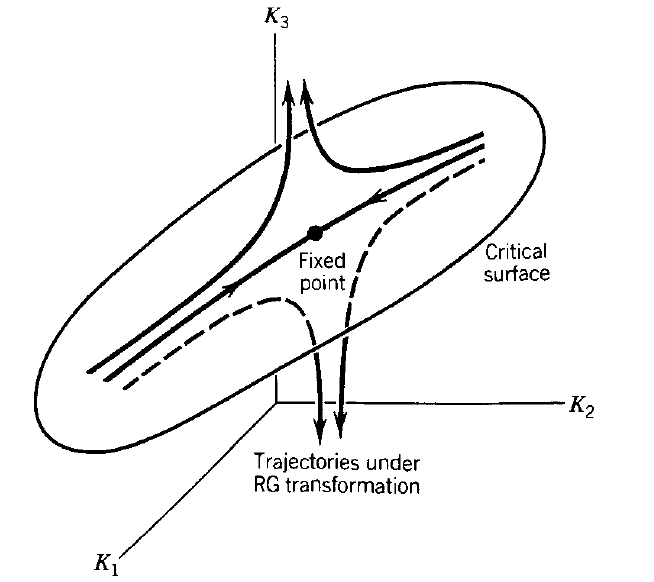
\includegraphics[width=0.7\textwidth]{criticalsf}
    \caption{Critical surface}
\end{figure}

If the critical surface has "codimension" $k$: 
\begin{enumerate}
    \item There are $k$ relevant perturbations 
    \item Experimentalists must tune $k$ parameters to acoss critical surface
\end{enumerate}

\section{Extensions}

We can experiment with modifications 
\begin{itemize}
    \item Square lattice
    \item have the possibility of "vacancies", $S = \pm 1, 0$ (we had a term in $S_i^2$ to the Hamiltonian)
    \item models with more states (ex Potts model, percolation)
    \item have boundaries, boundary conditions
\end{itemize}

\section{Symmetries and RG flows}
Recall Ising $\mathbb{Z}_2$ symmetry. 
\begin{enumerate}
    \item $\mathbb{Z}_2$-even couplings: $K\sum_{<ij>}S_iS_j$, etc 
    \item $\mathbb{Z}_2$-odd couplings: $K\sum_{i}S_i$, etc 
\end{enumerate}
Linearized RG equation 
\begin{equation}
    \delta K' = T \delta K  + O(\delta K^2)
\end{equation}
Previously $\underline{\delta K} = (\delta K, h)$
\begin{equation}
    T = \begin{pmatrix}
        b^{y_t} & 0 \\ 0 & b^{y_h}
    \end{pmatrix}
\end{equation}
More generally (more couplings), we have two blocks 
\begin{equation}
    T = \begin{pmatrix}
        \square & 0 \\ 0 & \square
    \end{pmatrix}
\end{equation}
associated to the even and odd sectors. There is a hierarchy of eigenvalues in each sector. There is a theorem which states there is only one relevant parameter per sector?

\subsection{Emergent symmetries}
RG preserves symmetries of $\mathcal{H}$ (should not lose a symmetry by zooming out). However, RG might generate new symmetries asymptotically (at fixed points). For exemple, conformal symmetry is emergent in critical ising model. \par \medskip 

\subsection{$\mathbb{Z}_2$ as an emergent symmetry}

Recall: $\mathbb{Z}_2$ symmetry means $\mathcal{H}[S] = \mathcal{H}[-S]$. \par \medskip 

In 3D, the Ising model has only 2 relevant perturbations, $\delta T$ and $h$. \par \medskip 

Interesting consequence for models that do not have microscopic $\mathbb{Z}_2$ but which have 2 experimental tuning parameters. Even though we cannot reach the critical point directly (we cannot have the $\mathbb{Z}_2$ symmetry microscopically), we can fix ourselves on the critical surface, which will flow to the critical point (we will have the $\mathbb{Z}_2$ symmetry macroscopically). 

\end{document}